\chapter{Tercera Iteración: El Emulador y los editores}

Como se explica en el la subsección \ref{metodologiadedesarrollo}, en la que se expone la metodología de desarrollo utilizada para el proyecto, este sufre de tres grandes iteraciones para su completitud. En esta sección se explican los detalles implementados en la tercera iteración, es decir, la generación de un emulador de juegos e eAdventure, utilizando el núcleo de ejecución \textit{Runner} explicado en la sección \ref{runnerit2}, y el modelo de datos de eAdventure explicado en \ref{coreit2}; además de la generación de editores para el editor de uAdventure desarrollado por Piotr Marszal. 

\section{El Emulador de Juegos}

Uno de los principales problemas de todo software consiste en que, el presupuesto que se invierte en el desarrollo de dicho software, no debe invertirse por completo en su desarrollo, pues la vida útil del mismo durará varios años más, en los que debe haber un mantenimiento y soporte para dicho software. El software producido por eAdventure, en muchos casos, hace años que dejó de tener soporte, pues no sólo los desarrolladores abandonaron los proyectos, sino que eAdventure no sufre ninguna actualización desde el 29 de Octubre de 2012, y todos los errores que han surgido, y los problemas de soporte que tiene en diferentes dispositivos han limitado la vida útil del software producido con eAdventure, y su ciclo de vida.

uAdventure, construido sobre Unity3D permite abrir proyectos de eAdventure, y videojuegos ya generados, dando la posibilidad de modificarlos, y probarlos sobre el nuevo núcleo de ejecución, ampliando y simplificando el ciclo de vida del videojuego. Tras haber abierto dicho juego, mediante las herramientas de compilación de Unity3D, se puede generar un paquete standalone con el juego en su interior.

No obstante, muchos proyectos han sido completamente abandonados, y es posible que nadie decida transformar un juego, o que, por desconocimiento de su existencia, no se transforme a uAdventure. Por todo ello, este framework puede ser compilado en sí mismo como un emulador de juegos de eAdventure, permitiendo al usuario explorar su sistema de ficheros, e importar de forma sencilla aquellos juegos que desee jugar.

Este emulador evoluciona de una prueba incluida en la clase controladora del juego en el prototipo generado en la primera iteración. Esto consistía en permitir al usuario seleccionar un juego de una lista de juegos disponibles en lugar de lanzar directamente un juego especificado en la clase controladora. En este primer prototipo la interfaz era muy sencilla, sin opciones, y no permitía técnicamente importar juegos, sino que debían de importarse descomprimiendo los juegos en una carpeta determinada del sistema de ficheros. Además, incluía un diálogo de carga que mostraba el progreso de la carga del juego.

Esta primera versión del emulador se muestra en la figura \ref{betaemuit3}.

\begin{figure}[htb]
	\centerline{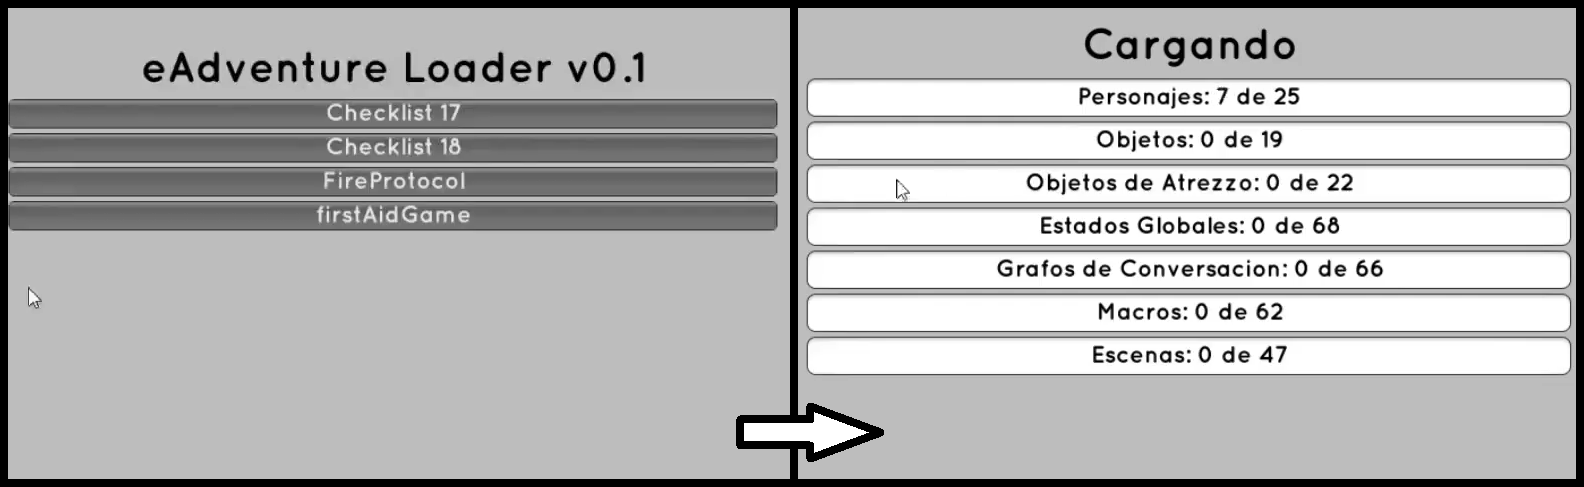
\includegraphics[height=2in]{figures/it3/betaemu.png}}
	\caption[Primer prototipo - Emulador]{La parte de la izquierda muestra el menú principal del primer prototipo del emulador. Una vez seleccionado un juego, se mostraba un diálogo de carga como el que se ve en la parte derecha.}
	\label{betaemuit3}
\end{figure}

No obstante, y dado que esta primera versión del emulador era insuficiente, además de que el diálogo de carga de ficheros no permitía ser ejecutado si se utiliza el sistema de carga de recursos de Unity3D, \textit{Resources.Load()}, este emulador evolucionó en 5 vistas:

\begin{itemize}
	\item \textbf{Menú Principal}: El menú es la puerta de entrada al emulador. Cuando se pone en funcionamiento muestra en el centro un catálogo de juegos instalados, si los hay. Pulsando sobre cualquiera de estos juegos comienza la ejecución del mismo. Finalmente, en la parte inferior de la vista hay 3 botones que permiten acceder a más vistas del emulador. Cada juego presentado en el menú principal tiene un icono que lo representa. La obtención de dicho icono se hace explorando los archivos incluidos dentro del directorio \textit{/gui/} en busca de un fichero llamado "standalone\_game\_icon.png", si dicho fichero no existe, se selecciona el icono de la versión de eAdventure con la que fue generado dicho juego, incluido también en el mismo directorio.

\begin{figure}[h!]
	\centerline{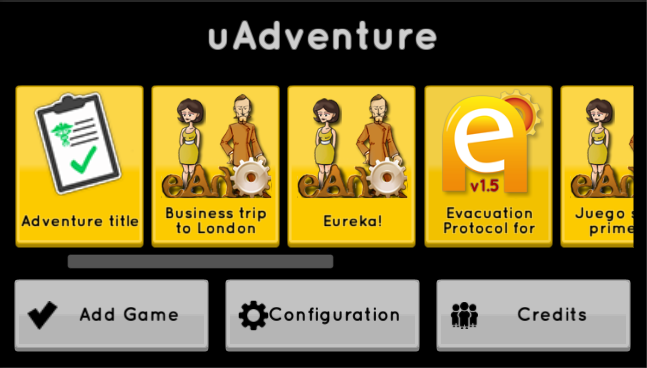
\includegraphics[height=2.5in]{figures/it3/emu-main.png}}
	\caption[Menu Principal - Emulador]{Vista del menú principal del emulador de uAdvneture.}
	\label{emumainit3}
\end{figure}


	\item \textbf{Explorador de Archivos}: Dado que Unity no provee, en tiempo de ejecución, de una manera de seleccionar un fichero del sistema de archivos, se ha implementado desde cero un explorador de archivos. Este permite navegar por carpetas, las cuales se ven en un color amarillo, y seleccionar juegos para ser añadidos. Estos juegos se representan con el icono de un mando de videojuegos, y con un color azul. Tras seleccionar un juego se puede pulsar el botón \textit{Add Game}, que lanza la vista que se presenta a continuación.

\begin{figure}[h!]
	\centerline{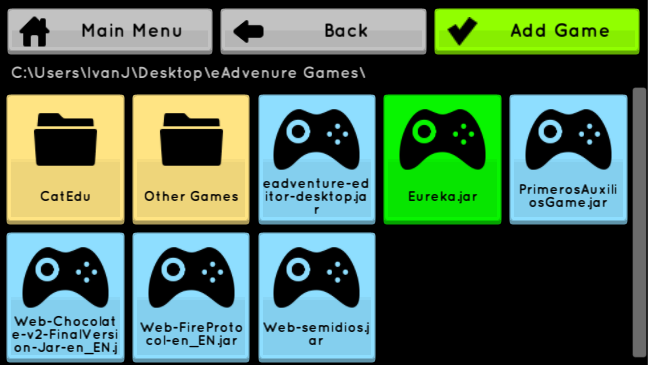
\includegraphics[height=2.3in]{figures/it3/emu-file.png}}
	\caption[Explorador de Archivos - Emulador]{Vista del explorador de archivos del emulador de uAdventure.}
	\label{emufileit3}
\end{figure}

	\item \textit{Importador de juegos}: Pese a que esta sea una de las vistas más sencillas, pues únicamente muestra un texto y una pequeña animación de tres puntos moviéndose, tras esta animación se encuentra el proceso de importado del juego. En el que se descomprimen las partes necesarias, y se borran algunos elementos tras su descompresión. Como se explicó en la sección \ref{resourcemanagerit2}, la transformación de los vídeos se realizaría en esta escena.
	
\begin{figure}[h!]
	\centerline{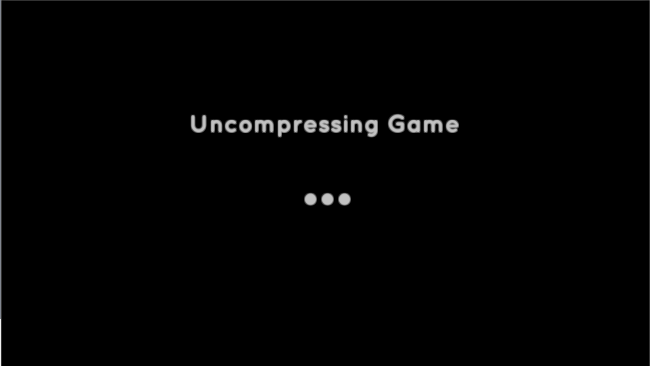
\includegraphics[height=2.3in]{figures/it3/emu-loader.png}}
	\caption[Importador de Juegos - Emulador]{Vista del importador de juegos del emulador de uAdventure.}
	\label{emuloaderit3}
\end{figure}
	
	\item \textit{Configuración}: La ventana de configuración provee al usuario de la capacidad de poder modificar el funcionamiento del intérprete, pudiendo configurar tres apartados: Gráficos, Sonido y Otros. Dentro del apartado gráfico se permite la posibilidad de deshabilitar los \textit{Shaders} explicados en la sección \ref{apearanceseccionit2}, así como deshabilitar los vídeos, o las animaciones. Dentro del apartado de sonido se permite configurar el uso de audio, así como su volumen y si se desea, forzar el uso de \textit{Text To Speech}, texto hablado. Finalmente, en el apartado de otras configuraciones, se permite modificar la velocidad del texto en las burbujas, así como la posibilidad de dehabilitar RAGE, o la persistencia de ficheros multimedia, para reducir el uso de memoria de la aplicación.
	
\begin{figure}[h!]
	\centerline{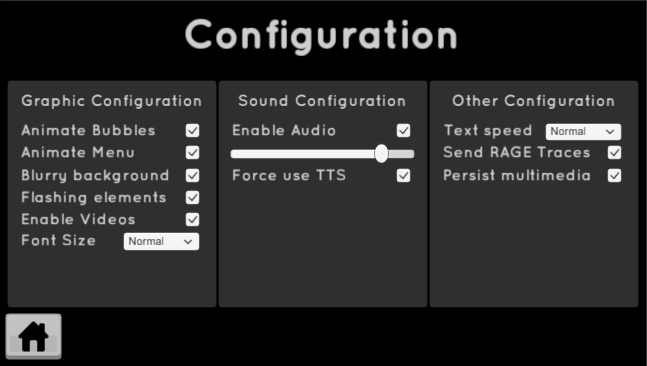
\includegraphics[height=2.3in]{figures/it3/emu-config.png}}
	\caption[Configuración - Emulador]{Vista de configuración del emulador de uAdventure.}
	\label{emuconfigit3}
\end{figure}
	
	\item \textit{Créditos}: La vista de créditos contiene el listado de las personas que han participado, dirigido o realizado aportaciones tanto a uAdventure como a eAdventure.
	
\begin{figure}[h!]
	\centerline{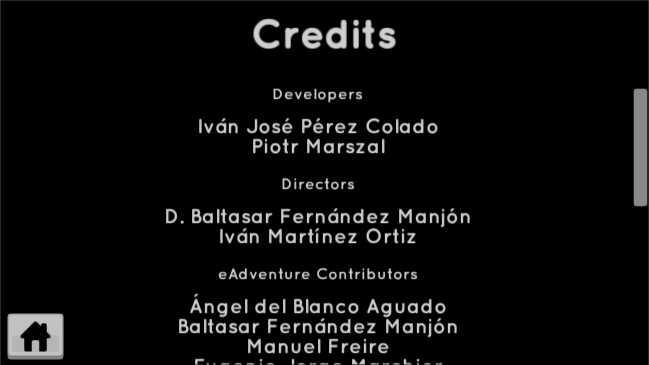
\includegraphics[height=2.3in]{figures/it3/emu-credits.png}}
	\caption[Créditos - Emulador]{Vista de los créditos presentados en el emulador de uAdventure.}
	\label{emucreditsit3}
\end{figure}

\end{itemize}





